\documentclass{article}[18pt]
\ProvidesPackage{format}
%Page setup
\usepackage[utf8]{inputenc}
\usepackage[margin=0.7in]{geometry}
\usepackage{parselines} 
\usepackage[english]{babel}
\usepackage{fancyhdr}
\usepackage{titlesec}
\hyphenpenalty=10000

\pagestyle{fancy}
\fancyhf{}
\rhead{Sam Robbins}
\rfoot{Page \thepage}

%Characters
\usepackage{amsmath}
\usepackage{amssymb}
\usepackage{gensymb}
\newcommand{\R}{\mathbb{R}}

%Diagrams
\usepackage{pgfplots}
\usepackage{graphicx}
\usepackage{tabularx}
\usepackage{relsize}
\pgfplotsset{width=10cm,compat=1.9}
\usepackage{float}

%Length Setting
\titlespacing\section{0pt}{14pt plus 4pt minus 2pt}{0pt plus 2pt minus 2pt}
\newlength\tindent
\setlength{\tindent}{\parindent}
\setlength{\parindent}{0pt}
\renewcommand{\indent}{\hspace*{\tindent}}

%Programming Font
\usepackage{courier}
\usepackage{listings}
\usepackage{pxfonts}

%Lists
\usepackage{enumerate}
\usepackage{enumitem}

% Networks Macro
\usepackage{tikz}


% Commands for files converted using pandoc
\providecommand{\tightlist}{%
	\setlength{\itemsep}{0pt}\setlength{\parskip}{0pt}}
\usepackage{hyperref}

% Get nice commands for floor and ceil
\usepackage{mathtools}
\DeclarePairedDelimiter{\ceil}{\lceil}{\rceil}
\DeclarePairedDelimiter{\floor}{\lfloor}{\rfloor}

% Allow itemize to go up to 20 levels deep (just change the number if you need more you madman)
\usepackage{enumitem}
\setlistdepth{20}
\renewlist{itemize}{itemize}{20}

% initially, use dots for all levels
\setlist[itemize]{label=$\cdot$}

% customize the first 3 levels
\setlist[itemize,1]{label=\textbullet}
\setlist[itemize,2]{label=--}
\setlist[itemize,3]{label=*}

% Definition and Important Stuff
% Important stuff
\usepackage[framemethod=TikZ]{mdframed}

\newcounter{theo}[section]\setcounter{theo}{0}
\renewcommand{\thetheo}{\arabic{section}.\arabic{theo}}
\newenvironment{important}[1][]{%
	\refstepcounter{theo}%
	\ifstrempty{#1}%
	{\mdfsetup{%
			frametitle={%
				\tikz[baseline=(current bounding box.east),outer sep=0pt]
				\node[anchor=east,rectangle,fill=red!50]
				{\strut Important};}}
	}%
	{\mdfsetup{%
			frametitle={%
				\tikz[baseline=(current bounding box.east),outer sep=0pt]
				\node[anchor=east,rectangle,fill=red!50]
				{\strut Important:~#1};}}%
	}%
	\mdfsetup{innertopmargin=10pt,linecolor=red!50,%
		linewidth=2pt,topline=true,%
		frametitleaboveskip=\dimexpr-\ht\strutbox\relax
	}
	\begin{mdframed}[]\relax%
		\centering
		}{\end{mdframed}}



\newcounter{lem}[section]\setcounter{lem}{0}
\renewcommand{\thelem}{\arabic{section}.\arabic{lem}}
\newenvironment{defin}[1][]{%
	\refstepcounter{lem}%
	\ifstrempty{#1}%
	{\mdfsetup{%
			frametitle={%
				\tikz[baseline=(current bounding box.east),outer sep=0pt]
				\node[anchor=east,rectangle,fill=blue!20]
				{\strut Definition};}}
	}%
	{\mdfsetup{%
			frametitle={%
				\tikz[baseline=(current bounding box.east),outer sep=0pt]
				\node[anchor=east,rectangle,fill=blue!20]
				{\strut Definition:~#1};}}%
	}%
	\mdfsetup{innertopmargin=10pt,linecolor=blue!20,%
		linewidth=2pt,topline=true,%
		frametitleaboveskip=\dimexpr-\ht\strutbox\relax
	}
	\begin{mdframed}[]\relax%
		\centering
		}{\end{mdframed}}
\lhead{Software Methodologies - Image Processing}


\begin{document}
\begin{center}
\underline{\huge Point intensity transforms for contrast enhancement}
\end{center}
\section{Functional point transforms}
Processing each pixel value, p, individually using a mathematical function
$$p'=f(p)$$
as a point transform operator transforms the image from one state to another
\begin{center}
	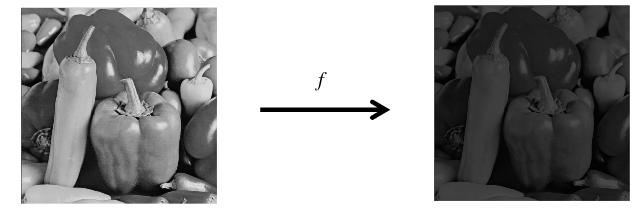
\includegraphics[scale=0.7]{functional}
\end{center}
Also known as intensity transform functions
\section{Image enhancement}
Goal: make the image look better so we can view and process the visual information with greater clarity\\
\\
Image enhancement is subjective. It depends on
\begin{itemize}
	\item The information required by the visual task
	\item The physical characteristics of the image
	\item The user's prior knowledge/experience
	\item The user's intuition and judgement
\end{itemize}
Evaluation methodology: perceived quality of results\\
\\
Common poor image characteristics: poor lighting and noise
\section{Dynamic range}
\begin{defin}[Range of a sensor]
The set of all possible intensity values of the images it captures
\end{defin}
A good image should utilise the full (or most of the) sensor's range
\begin{defin}[Dynamic range of a sensor]
The largest (possible) signal value divided by the smallest (possible) signal value
\end{defin}
Increasing the dynamic range improves contrast
\section{Conventions}
Pixels can either be represented as:
\begin{itemize}
	\item Floats from 0 to 1
	\item Integers from 0 to 255
\end{itemize}
\section{Logarithmic transform}
The logarithmic transform replaces each pixel value with its logarithm
\[
I_{\text {output}}(i, j)=\log I_{\text {input}}(i, j)
\]
In practice, we control the range using the function:
\[
I_{\text {output}}(i, j)=c \cdot \log \left[1+\left(e^{\sigma}-1\right) I_{\text {input}}(i, j)\right]
\]
with scaling parameters $\sigma$ and c
$\sigma$ controls the range of values onto which the logarithmic function is applied\\
\\
c normalises the output to the range [0,255]. That is,
$$c=\dfrac{255}{R}$$
Where R is the maximum of
$$\log \left[1+\left(e^{\sigma}-1\right) I_{\text {input}}(i, j)\right]$$
\begin{center}
	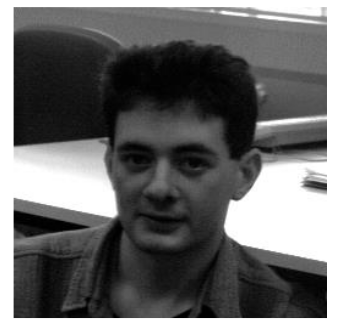
\includegraphics[scale=0.7]{log}
\end{center}
The dynamic range of this scene exceeded that of the sensor/camera (dark foreground - bright background)\\
\\
As a result of a (usually automatic) decision on the camera exposure, the dynamic range of the dark parts was compressed
\begin{center}
	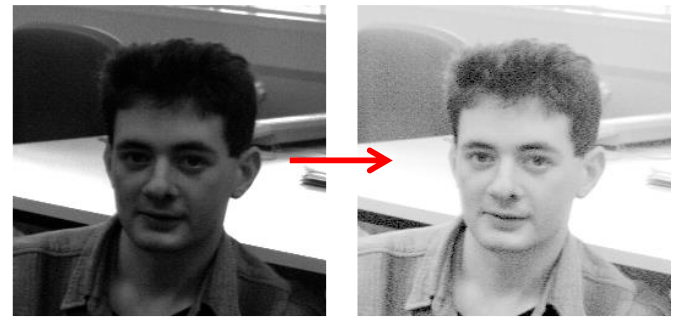
\includegraphics[scale=0.7]{log1}
\end{center}
The logarithmic transform in this example:
\begin{itemize}
	\item brightens the foreground (which consists of dark pixels) spreading low pixel values over a wider range
	\item compresses the background pixel range (the bright high values)
\end{itemize}
Applying the logarithmic transform yields poor results: information loss and worse visualisation
\section{Application: X-ray images}
X-ray sensors return values given by an exponential function
\[
I(i, j)=I_{o} \cdot \exp (-f(i, j))
\]
$I_o$ is the X-ray source intensity\\
f = material attenuating properties (object thickness and material density)\\
\\
The logarithmic transform cancels the exponent
\[
\log I_{o u t}=\log \left[I_{o} \cdot(\exp (-f(i, j))]\right.
\]
As a result, the image gives a linear mapping of the material properties
\section{Exponential transform}
The exponential transform is the inverse of the logarithmic transform\\
\\
It replaces each pixel value with its exponent
\[
I_{\text {output}}(i, j)=\exp \left(I_{\text {input}}(i, j)\right)
\]
In practice, we use a variable basis and scaling
\[
I_{\text {output}}(i, j)=\mathrm{c} \cdot\left[(1+\alpha)^{I_{\text {input}}(i, j)}-1\right]
\]
where $1+\alpha$ is the basis and c the scaling factor\\
\\
$I_{input}(i,j)=0$ gives
\[
I_{\text {output}}(i, j)=\mathrm{c} \cdot\left[(1+\alpha)^{I_{\text {input}}(i, j)}\right]=c
\]
We subtract 1 to prevent offset in output\\
\\
Basis $>1$ is required for functions suitable for out purpose (decrease the dynamic range of dark regions - increase the dynamic range of bight regions)
\begin{center}
	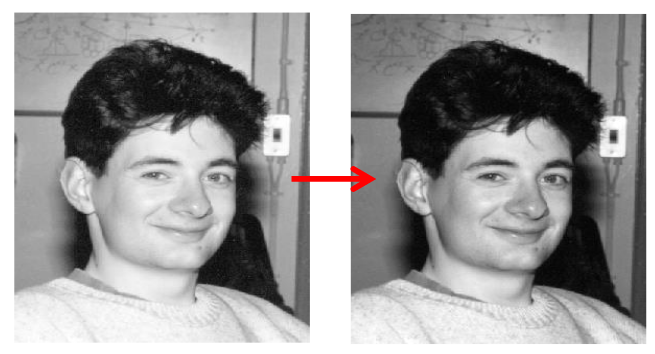
\includegraphics[scale=0.7]{exp}
\end{center}
The exponential transform decreases the dynamic range of dark regions whilst increasing the dynamic range in light regions\\
Enhances detail in high value (bright) areas
\section{Power-law ('raise to power') transform}
Raise each pixel value to a fixed power
\[
I_{\text {output}}(i, j)=c \cdot\left(I_{\text {input}}(i, j)\right)^{r}
\]
for $r>1$ it enhances (spreads) high value intensities whilst compressing low value intensities\\
\\
For $r<1$ it enhances (spreads) low value intensities whilst compressing high value intensities\\
\\
The 'power-law' transform has similar effect the logarithmic (when $r<1$) or to the exponential (when $r>1$)
\section{Application: gamma correction}
The power-law transform is used in digital photography to correct the tonality of an image\\
\\
r is traditionally called the gamma value, and the process gamma correction\\
\\
The transform $f(x)=x^\gamma$ with $\gamma<1$ weights the intensities towards higher (brighter) values
\begin{itemize}
	\item an underexposed photo can be corrected using gamma correction with $\gamma<1$
\end{itemize} 
The transform $f(x)=x^y$ with $\gamma>1$ weights the intensities toward lower(darker) values
\begin{itemize}
	\item An overexposed photo can be corrected using gamma correction with $\gamma>1$
\end{itemize}
\begin{center}
	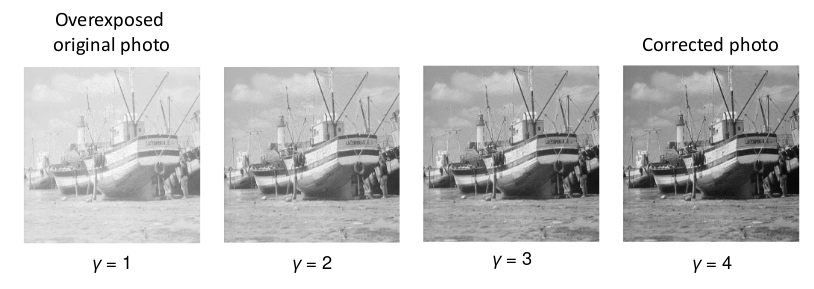
\includegraphics[scale=0.7]{gamma}
\end{center}

\end{document}